% Please write one sentence per line! (easier for version control)

\documentclass[10pt, a4paper]{article}
\usepackage{lrec2006}
\usepackage{graphicx}
\usepackage{linguex}
\usepackage{amssymb}

\usepackage{todonotes}
% To hide all notes use 
%\usepackage[disable]{todonotes}


\title{Towards text mining in earth science:\\
extraction of quantitative variables and their relations}

\name{Author1, Author2, Author3}

\address{ Affiliation1, Affiliation2, Affiliation3 \\
               Address1, Address2, Address3 \\
               author1@xxx.yy, author2@zzz.edu, author3@hhh.com\\}


\abstract{
This paper addresses text mining in the cross-disciplinary domain of earth science, environmental science and climate science.
It is motivated by the desire for literature-based knowledge discovery from scientific publications.
The particular goal is to automatically extract relations between quantitative variables from raw text.
This results in rules of the form ``If variable X increases, than variable Y decreases''.    
As a first step in this direction, an annotion scheme is proposed to capture the events of interest -- those of change, cause, correlation and feedback -- and the entities involved in them -- quantitative variables.
Its purpose is to serve as an intermediary step in the process of rule extraction.
It is shown that the desired rules can indeed be automatically extracted from annotated text.
A number of open challenges are discussed, including automatic annotation, normalization of variables, reasoning with rules in combination with domain knowledge and the need for meta-knowledge regarding context of use.
\\ \newline 
\Keywords{Text Mining, Literature-based Knowledge Discovery, Earth Science, Environmental Science, Climate Science, Corpus Annotation, Relation Extraction, Event Extraction}}

\newcommand{\tag}[1]{\textsc{#1}}

% Define your own todo notes here, like 
% \newcommand{\XX}[1]{\todo[inline,author=XX,color=YY]{#1}}
\newcommand{\EM}[1]{\todo[inline,author=EM,color=yellow]{#1}}
\newcommand{\EA}[1]{\todo[inline,author=EA,color=green]{#1}}
\newcommand{\MVA}[1]{\todo[inline,author=MVA,color=blue]{#1}}
\newcommand{\PO}[1]{\todo[inline,author=PO,color=pink]{#1}}



\begin{document}

\maketitleabstract

%=============================================================================
\section{Introduction}
%=============================================================================

One of the characteristics of the cross-disciplinary fields of earth science, environmental science and climate science is the existence of many different processes that affect each other in direct and indirect ways, resulting in highly complex systems.
In climate science, for example, \emph{climate feedback} is defined as ``An interaction in which a perturbation in one climate quantity causes a change in a second, and the change in the
second quantity ultimately leads to an additional change in the first. 
A negative feedback is one in which the initial perturbation is weakened
by the changes it causes; a positive feedback is one in which the initial
perturbation is enhanced.'' \cite{stocker2013climate}.
Indentifying such feedback processes is generally considered a crucial step in understanding and predicting phenomena like global warming.

Unfortunately much potential knowledge regarding processes and their interactions is hidden in the scientific literature, scattered over journals catering to different scientific communities with relatively little communication among them.
Given the vast and constantly growing nature of this body of literature, it is indeed hard for individual researchers to keep track of all relevant publications in their field of expertise, let alone of those in related or even more distant areas.   

Text mining of scientific literature may contribute to alleviating this problem \cite{Etzioni2011Search} .
Earth, environmental and climate science may all benefit from automatic retrieval and extraction of processes and their interactions from scientific publications.
The extracted information can be indexed, thus allowing researchers to search for interactions between processes in a much more effective way than with conventional keyword-based search engines.
In addition, this structured information can be used for inference in discovery support systems.
For example, pairs of cause and effect processes can be chained together, possibly in combination with existing domain knowledge, in order to suggest hypotheses about indirect interactions or feedback loops or to point out contradictory findings.

Curently text mining in earth science, climate science and environmental science appears to be virtually non-existent. 
As a first step in this direction, this paper explores the possibities for automatic extraction of relations between quantitative variables from raw text.
The desired rules are of the type: ``If variable X increases, than variable Y decreases''.
Following the lead of text mining initiatives in biomedicine \cite{Kim2009Overview}, we explore manual text annotation for creating annotated corpora, which can be used to train classifiers for automatic annotation, and ultimately automatic rule extraction. 
In Section~\ref{sec:annot}, an annotion scheme is proposed to annotate the events of interest, namely, those of change, cause, correlation and feedback, as well as the entities involved in them.
Its purpose is to serve as an intermediary step in the process of rule extraction.
It is shown in Section~\ref{sec:extraction} that such rules can indeed be automatically extracted from annotated text.
Section~\ref{sec:discussion} discusses a range of open challenges, including automatic annotation, normalization of variables, reasoning with rules in combination with domain knowledge and the need for meta-knowledge regarding context of use.
The final Section~\ref{sec:conclusion} closes with conclusions and future work.
Prior to that, the next Section starts off with discussing related work on event extraction and causal relation extraction.


%=============================================================================
\section{Related work}
%=============================================================================
\label{sec:related}

\todo[inline]{Sharpen: focus on why our work is new/different from related work}

\subsection{Literature-based knowledge discovery}

In a cross-disciplinary field, as knowledge regarding concepts and their relations are scattered across scientific communities with a limited degree of interaction, it is likely that there exists inferences that can be made on basis of existing knowledge, but have not been made, because no single research group has had the required knowledge to make the inference. 
\newcite{Swanson1986Undiscovered} labelled these potential inferences \emph{undiscovered public knowledge}, and made the claim that they are ubiquitous in science. 
As an example, he hypothesized that fish oils can cure Raynaud's disease by combining two publicly available statements: 1) Fish oils reduce blood viscosity, 2) patients with Raynaud's disease tend to exhibit high blood viscosity \cite{Swanson1986Fishoil}. 
This method of inferring hypotheses of the form $A \to C$ based on publicly available statements $A \to B$ and $B \to C$ has been termed \emph{Swanson linking}\footnote{In the Swanson linking paradigm, the operator $\to$ is not interpreted as a logical conditional, but rather as an abstract causal or correlative relation between the terms. The conclusion $A \to C$ is therefore not logically sound, but has nevertheless been showed to give empirically useful results.}. 

The discoveries of Swanson prompted a line of research into methods for computer support in the identification of undiscovered public knowledge, an area which has been labelled Literature-based discovery (LBD). 
Most LBD methods are based on Swanson linking, and use term co-occurrence frequencies to detect relations of the type $A \to B$. 
Terms are usually extracted as n-grams from the text \cite{Lindsay1999LBDLexicalStat} or taken from a controlled vocabulary or ontology \cite{Weeber2001ConceptsInLBD}.

Recently, co-occurrence based methods have come under critique for yielding imprecise results, as they fail to exploit the true structure of knowledge contained in scientific literature.
\newcite{Hristovski2008NLPinLBD} therefore advocate a text mining based approach, where the relation extraction is used to discover relations between two concepts.
LBD efforts have traditionally been undertaken in the biomedical domain, and have therefore benefited from existing biomedical NLP tools such as SemRep\footnote{http://semrep.nlm.nih.gov/}.
Application of text mining-based LBD techniques to less resourced domains would however require the development or adaptation of NLP tools, a goal which the current paper can be considered the first step towards. 

\subsection{Relation extraction}

For an NLP system to support LBD, automatic extraction of relations from text is required. In relation extraction, the causal relation is one of the most common target relations. 
Causal relations are used in a range of tasks such as question answering, as well as LBD. 
In the work by \cite{Mihaila2013}, several machine learning algorithms are applied to recognize causality triggers such as "therefore", "because", "as a result of" etc..
The approach is tested on BioCause and BioDRB corpora, which consist of articles with manually annotated causal relations between named entities in the biomedical domain. 
Machine learning approach has also been applies by \cite{Pechsiri2010a} to extract causal relations in the agricultural domain. 
These relations are then used to construct explanation knowledge graphs that represent the domain knowledge.

Causal relations is not the only type of relations that can be used for LBD purposes. 
Other, more fine-grained types of relations has been identified as well. In the work by \cite{Zambach2010Lexical}, the authors identify and analyse verbs that express regulation relations, positive and negative, between processes and substances in biomedical domain. 
They propose that this knowledge can be used for automatic annotation of such relations in text. A somewhat similar types of relations has been proposed by \cite{Hashimoto2012Excitatory}. 
They identify excitatory, inhibitory and neutral relations with corresponding set of extraction templates. 
More templates are acquired automatically by a bootstrapping process. 
Excitatory relations are then used for extraction of contradictions, causality relations and generation of causality hypothesis.

The current task differs from other text mining tasks in the type and structure of target relations. 
In most text mining tasks, the goal is to extract binary relations holding between two objects such as $CAUSE(x,y)$, while we seek to extract variables, change events involving the variables, and causality/correlation relations holding between change events.  

%=============================================================================
\section{Annotation}
%=============================================================================
\label{sec:annot}

\subsection{Procedure}

The data consisted of 12 abstracts (2369 words) from recent, high-quality scientific journal publications about the relation between climate and ocean changes. 
These were selected by our domain expert (author MVA) as a reasonably representative sample of the text type in the targeted area, comprissing multi-disciplinary work in marine biology, marine science, oceanography, environmental science, climate science, biogeoscience and geophysics.
Text was automatically extracted from PDF files.
Abstracts were manually extracted, tokenized and split into sentences, also allowing for manual correction of minor PDF-to-text conversion errors.

Annotation was carried out using the Brat annotation tool \cite{stenetorp2012}.
The annotion scheme described below was developed in an iterative fashion in close colaboration with our domain expert.
It is inspired by annotation efforts in the biomedical domain such as the GENIA corpus \cite{Kim2003GENIA} and the corpora used in the BioNLP shared tasks on event extraction \cite{Kim2009Overview}.
It covers a particular type of events -- those of change, cause, correlation and feedback -- and the entities involved in them -- quantitative variables.
The primary reason of annotation is not to analyse the text according to some linguistic formalism or theory, or to follow some knowledge representation formalism or ontological theory.
Instead the purpose of the annotation is rather pragmatic: to serve as an intermediary step in the process of extracting rules about the relation between quantitative variables from raw text.      
 
\subsection{Annotation scheme}

The resulting annotation scheme involves one type of entity (variable), several types of events (change, increase, decrease, cause, correlate, feedback) and some basic logic structure (and/or, negation).  


\subsubsection{Variables}

A quantitative variable is an entity that can be counted or measured.
Its value can be naturally expressed by a number such as a count, a ratio, a percentage or a scalar (quantity of units).
It can be regarded as a (potential) quantitative variable in an experiment or a model. 
Not every variable in the text is labeled as such.
To save annotation time and effort, only those variables related to a change are annotated.
The  direction of change can be positive (increasing), negative (decreasing) or unspecified (either increasing or decreasing), but there must always be a clear cue in the text that the variable is involved in some change. 
Examples of changing, increasing and decreasing variables respectively:

\ex.
  \a. significant changes in [\emph{surface ocean pH}]
  \b. rise in [\emph{atmospheric CO2 levels}]
  \c. decline in [\emph{marine primary production}]

In contract, the text spans in \Next are not annotated as variables.

\ex.
  \a. *[\emph{carbon dioxide}] and [\emph{light}] are two major prerequisites of photosynthesis
  \b. *changes in [\emph{the network of global biogeochemical cycles}] 
  \c. *The concentrations of [\emph{DFe}] and [\emph{TaLFe}] were relatively high

The text spans in \Last[a] are measurable, in principle at least, but there is no textual cue in the context indicating that they are subject to change. 
The text span in \Last[b] admittedly identifies something that is changing, but it is an abstraction -- not something that can be measured and naturally expressed through a number. 
The ones in \Last[c] express a static state rather than a dynamic event.
The reason for excluding cases like these is that they do not lead to useful rules about the relation between quantitative variables.

Variables must be indicated as precisely as possible, that is,including any relevant specifications, modifications or conditions. So instead of \Next[a], \Next[b] is prefered.

\ex.
  \a. *a difference in [\emph{carbon concentration}] between the ocean surface and the deep waters
  \b. a difference in [\emph{carbon concentration between the ocean surface and the deep waters}]

The choice is motivated by the idea that, given a syntactic parse, it is usually easier to generalize a complex argument by stripping modifiers than the other way around.  

Variables are tagged with the label \tag{Variable}. It is most likely advantaguous to distinguish different subclasses of variables. Currently we are not concerned with this. 
However, we do not exclude the possibility of a more fine-grained annotation at a later stage. 


\subsubsection{Change, Increase and Decrease}

A change is an event in which the value of a quantitative variable is changing.
The direction of change can be positive (increasing), negative (decreasing) or unspecified (either increasing or decreasing), but there must always be a clear cue in the text that the variable is involved in a change.
This is referred to as the \emph{trigger} for the event.

Examples of triggers for event types of change, increase and decrease are:

\ex.
  \a. [\emph{regional changes}] in phytoplankton
  \b. [\emph{addition of}] labile dissolved organic carbon
  \c. [\emph{to slow down}] calcification in corals

Changes must apply to a variable; hence the text span in \Next does not trigger a

\ex. *marine primary production is sensitive to climate [\emph{variability and change}]

Events of increase, decrease and undirected changes are tagged as \tag{Increase}, \tag{Decrease} and \tag{Change} respectively. 
Events are related to variables through thematic roles, which specify the different participants in the event. 
Change events must always have a \tag{Theme} role that is filled by the variable that is changing.
Typical annotation examples are therefore:\footnote{We use labeled brackets to denote enitities, events or thematic roles, depending on the context of discussion.}

\exi.
  \a. [\tag{Decrease} reduced] [\tag{Theme} calcite production]
  \b. [\tag{Change} significant changes in] [\tag{Theme} surface ocean pH]

In addition, they can optionally have an \tag{Agent} role or a \tag{Co-theme} role, which will be explained in the next Section.

Change events can also function as Cause/Correlate events, as will be described in the next Section, in which case they take an AGENT or CO-THEME role as well.


\subsubsection{Cause}

Cause events involve a pair of changes where the first change causes the second change.
Since a change event involves a changing variable, as its theme, causal events thus express a causal relation between two changing variables. 
The trigger of a cause event is annotated with a \tag{Cause} tag.
Triggers are often verbs, but can also be adjectives (\emph{stimulatory}), adverbs (\emph{therefore}) or subjunctive phrases (\emph{due to}, \emph{in response to}) and other phrasal expression (\emph{has an effect on}).  

Cause events must always have two thematic roles: an \tag{Agent} identifying the cause and a \tag{Theme} identifying the effect. 
% Notice that causal relations are directional. 
% That if, if  A causes B, then it does not follow that B causes A.
Examples of cause events are:

\exi.
  \a. [\tag{Agent} rise in atmospheric CO2 levels] [\tag{Cause} \emph{causes}] [\tag{Theme} significant changes in surface ocean pH]
  \b. [\tag{Agent} Fe(III) addition in the presence of GA (FeGA)] [\tag{Cause} \emph{gave}] [\tag{Theme} higher Fe(II) concentration]
  \c. [\tag{Agent} diminished calcification] [\tag{Cause} \emph{led to}] [\tag{Theme} a reduction in the ratio of calcite precipitation to organic matter production]
% number of examples can be reduced

In many cases, a cause event and a change event share one and the same trigger, as in the following examples:

\exi.
  \a. [\tag{Agent} changes in the magnitude of total and export production] [\tag{Change} \emph{can strongly influence}] [\tag{Theme} atmospheric CO2 levels]
  \b. [\tag{Theme} calcification and net primary production] [\tag{Increase} \emph{ are significantly increased by}] [\tag{Agent} high CO2 partial pressures]
  \c. [\tag{Agent} addition of labile dissolved organic carbon] [\tag{Decrease}  \emph{reduced}] [\tag{Theme} phytoplankton biomass]

In \Last[a], \emph{can strongly influence} serves as the cue for a change event with variable \emph{atmospheric CO2 levels} as its theme. 
At the same time, it is the trigger for a cause event with agent \emph{ changes in the magnitude of total and export production} and theme \emph{atmospheric CO2 levels}.
In principle, both events can be annotated individually.  
However, in order to avoid a needlessly complex annotation, we choose to not annotate the cause event explicitly. 
Instead \emph{changes in the magnitude of total and export production} is given the role of agent in the change event. 
Presence of an agent role suffices to infer the cause event.
Two more instances of this pattern are shown in \Last[b] and \Last[c].

\EM{Describe exceptional cases of variable with implicit change}


\subsubsection{Correlate}

Correlate events involve a pair of changes where the first change correlates with the second change. 
Since a change event involves a changing variable, as its theme, correlate events thus express a correlation between two changing variables. 
That is, if one of them changes, the other changes along. 
Correlations  have two roles, \tag{Theme} and \tag{Co-theme}, both of which should be fulfilled by a change event (i.e. \tag{Increase}, \tag{Decrease} or \tag{Change}).
% or a quantitative variable (Variable)
Examples of correlate events:

\exi.
  \a. [\tag{Theme} reduced calcite production] [\tag{Correlate} \emph{ was accompanied by}] [\tag{Co-theme} an increased proportion of malformed coccoliths]
  \b. [\tag{Theme} carbon:nutrient ratio turns out to decrease] [\tag{Correlate}  \emph{with}] [\tag{Co-theme} increasing mixed-layer depth and temperature]
  \c. Here we report [\tag{Them}e reduced calcite production] [\tag{Correlate}  \emph{at}] [\tag{Co-theme} increased CO2 concentrations]
  \d. [\tag{Correlate} \emph{When}] [Co-theme bacterial growth rate was limited by mineral nutrients], [Theme extra organic carbon accumulated in the system]
%  \e. [\tag{Theme} regional changes in phytoplankton] [\tag{Correlate} coincide with] [\tag{Co-theme} observed changes in kril]

Notice that correlation can be triggered by a verb \Last[a], a preposition \Last[b-c] or an adverb/conjunction \Last[d].

Statistically speaking, correlation is not a directional relation, in contrast to causation. That is, if a change in variable A is correlated with a change in variable B, then it follows that a change in variable B is correlated with a change in variable A. However, in discourse there is often a distinction between a variable of interest (the dependent variable) and related variable (the independent variable). 
Thus even though strictly speaking there is no causal relation between the two variables, the text usually takes a particular perspective, suggesting one is more central than the other. 
By convention, the central variable is tagged as \tag{Theme}, whereas the other one is tagged as \tag{Co-theme}. 
The rule of thumb is that the co-theme is syntactically the argument of a preposition (e.g. \emph{with, at, under}) or an adverb/conjunction (e.g. \emph{when}).  

Occasionally correlations can hold between a change event and a variable, or even between two variables, rather than between to change events.
In these exceptional cases, we assume the variable is interpreted as changing (i.e. as being part of an implicit change event), because it is involved in a correlate event.
Two examples of this exceptional pattern are: 

\exi.
  \a. [\tag{Increase} Concentrations of DFe increased slightly] [\tag{Correlate} with]  [\tag{Variable} depth in the water column]
  \b. [\tag{Variable} growth rates in the high-CO2-grown cells] [\tag{Correlate} were related to] [\tag{Variable} light level]


In \Last[a], the role of co-theme is not taken by a change event, but by the variable \emph{depth in the water column}.
It is thus assumed that the depth in the water column is a changing variable in the correlation described.
Similarly, \Last[b] has both roles of the correlate event taken up by variables, which are therefore interpreted as subject to change.

\EM{Should we allow the same for \tag{Cause}? Check data} 
\EA{Perhaps we can move this discussion, together with the discussion of inherently changing variables (Ocean Acidification, etc), to a new sub-chapter about variables that are interpreted as changing without an explicit change?}

\subsubsection{Feedback}

Feedback loops are an important concept in climate science. An example is that of the relation between rising temperature and methane release: a rise in temperature causes more permafrost to melt, which causes more release of methane in the atmosphere (a ``green house'' gas), which causes further rising of the temperature, and so on.
However, explicit mentioning of feedback events in the text appears to be rare compared with the frequent occurrence of change events, so our proposal for annotation of feedbacks is currently based on only a couple of instances.
Feedback events hold between two variables, filling the roles of \tag{Theme} and \tag{Co-theme}, as exemplified below: 

\exi. our model suggests the existence of [\tag{+Feedback} a positive feedback between] [\tag{Theme} temperature] and [\tag{Co-theme} atmospheric CO2 content]

Analogously to change events, feedback events can positive (self-sustaining, self-enhancing), negative (self-stabilizing, self-diminishing) or of unspecified polarity.
Positive or negative feedback are annotated with an attributue whenever a trigger is present. 

\subsubsection{Referring expressions}

Referring expressions such as anaphoric expressions (e.g. \emph{it}, \emph{this}) and underspecified definite descriptions (e.g. \emph{the process}) are annotated only in so far as they play a thematic role in an event of interest. Consider the following narrative:

\exi. 
  \a.[s1:] Future shoaling of upper-mixed-layer depths will expose phytoplankton to [\tag{Increase} increased] [\tag{Theme} mean light intensities].
  \b.[s2:] [\tag{RefExp/Agent} \emph{This}] [\tag{Cause} may cause] [\tag{Decrease} a widespread decline in] [\tag{Theme} marine primary production]

The first sentence contains an \tag{Increase} event, which is referred to in the second sentence by means of the referring expression \emph{This}, establishing it as the cause for the\tag{Decrease} event.
The referring expressions must therefore be resolved in order to arrive at the rule an increase in mean light intensities causes a decrease in marine primary production.
In order to achieve this, such referring expressions are tagged as \tag{RefExp} and connected with their antecedent by means of a \tag{Coref} relation. 
  

\subsubsection{Combinations}

Variables or events can be combined through conjunction or disjunction.
Such combinations are labeled as \tag{And} or \tag{Or}, where their constituents fill the role of \tag{Part}.
In \Next[a], for example, the combination \tag{And} serves as the theme of the \tag{Increase} event.
Likewise, two increasing events are combined to serve as the theme in a causal event.

\exi.
  \a. [\tag{Increase} increasing [\tag{Part:Variable} mixed-layer depth] [\tag{Theme:And} and] [\tag{Part:Variable} temperature]  
  \b. [\tag{Cause} gave] [\tag{Part:Increase} higher ] Fe(II) concentration [\tag{Theme:And} and] [\tag{Part:Increase} higher] growth rate of phytoplankton

The alternative option in \Last[a] is to tag the whole combined phrase as a single variable.
We chose not do so because coordination is notoriously hard problem for syntactic parsers and any help from the annotation in resolving ambiguity should be exploited.
Notice also that a similar option is not availabe in \Last[b], as considering the whole combination as a single change event would result in loss of substantial information.


\subsubsection{Negation}

Events can carry a negation attribute to account for examples such as:

\exi.
  \a. TaLFe [\tag{Correlate+Neg} did \emph{not} show any consistent trend with] depth 
  \b. [\tag{Change+Neg} \emph{No} differences] in cellular organic carbon:nitrogen ratios were observed

Triggers for negation are currently not explicitly annotated.


%=============================================================================
\section{Rule extraction}
%=============================================================================
\label{sec:extraction}

The proposed annotation allows for autamatic extraction of rules about the relations between quantitative variables.
There are three main types of rules: causal rules, correlation rules and feedback rules.

Causal rules are of the type ``If variable X changes, than variable Y changes''.
An example of such rule its source text is shown in Figure~\ref{fig:ex1}.
The notation uses single arrows to denote changing variables, where `$\uparrow$' stands for 'increasing', `$\downarrow$' for 'decreasing' and `$\updownarrow$' for 'changing.'
Parts of combination are joined by `$\wedge$' and delimited by square brackets.
A causal relation is denoted by the double arrow `$\Longrightarrow$'.
Causal rules are basically extracted by looking for \tag{Cause} events, taking their \tag{Agent} and \tag{Theme} roles for cause and effect respectively.
Another source for causal rules is change events with both an \tag{Agent} and a \tag{Theme} role.
Notice that in Figure~\ref{fig:ex1}, interpreting combinations and resolving referring expressions to their antecedent takes some additional processing.
Another source for causal rules is change events with both \tag{Agent} and \tag{Theme} roles.

Correlation rules are of the type ``Changes in variable X correlate with changes in variable Y'', as exemplified in Figure~\ref{fig:ex2}.
The curly arrow `$\leadsto$' is used to indicate the relation between a independent and a dependent variable.
These rules are extracted from \tag{Corelate} events, using their \tag{Co-theme} role as the independent variable (LHS of the rule) and their \tag{Theme} role as the dependent variable (RHS of the rule). 

Feedback rules, an example of which is shown in Figure~\ref{fig:ex3}, are of the form: ``Changes in variable X feed back through changes in variable Y''.
The feedback relation is denoted by a double sided arrow `$\Longleftrightarrow$', optionally with a superscripted '+' or '-' for positive and negative feedback respectively.

Notice that conceptually a feedback relation is assumed to hold between changing events.
However, often there is no explicit trigger for a change event present in the text.
For example, in the annotation in Figure~\ref{fig:ex3}, both roles are filled by variables instead of change events.
Such variables are therefore 'promoted' to change events during rule extraction, resulting in `$\updownarrow$ temperature' and `$\updownarrow$ marine primary production'.
Similar promotion apply occassionaly to variables in events of change, cause or correlation.


\setlength{\fboxsep}{10pt}

\begin{figure*}
\begin{center}
\framebox[\textwidth]{
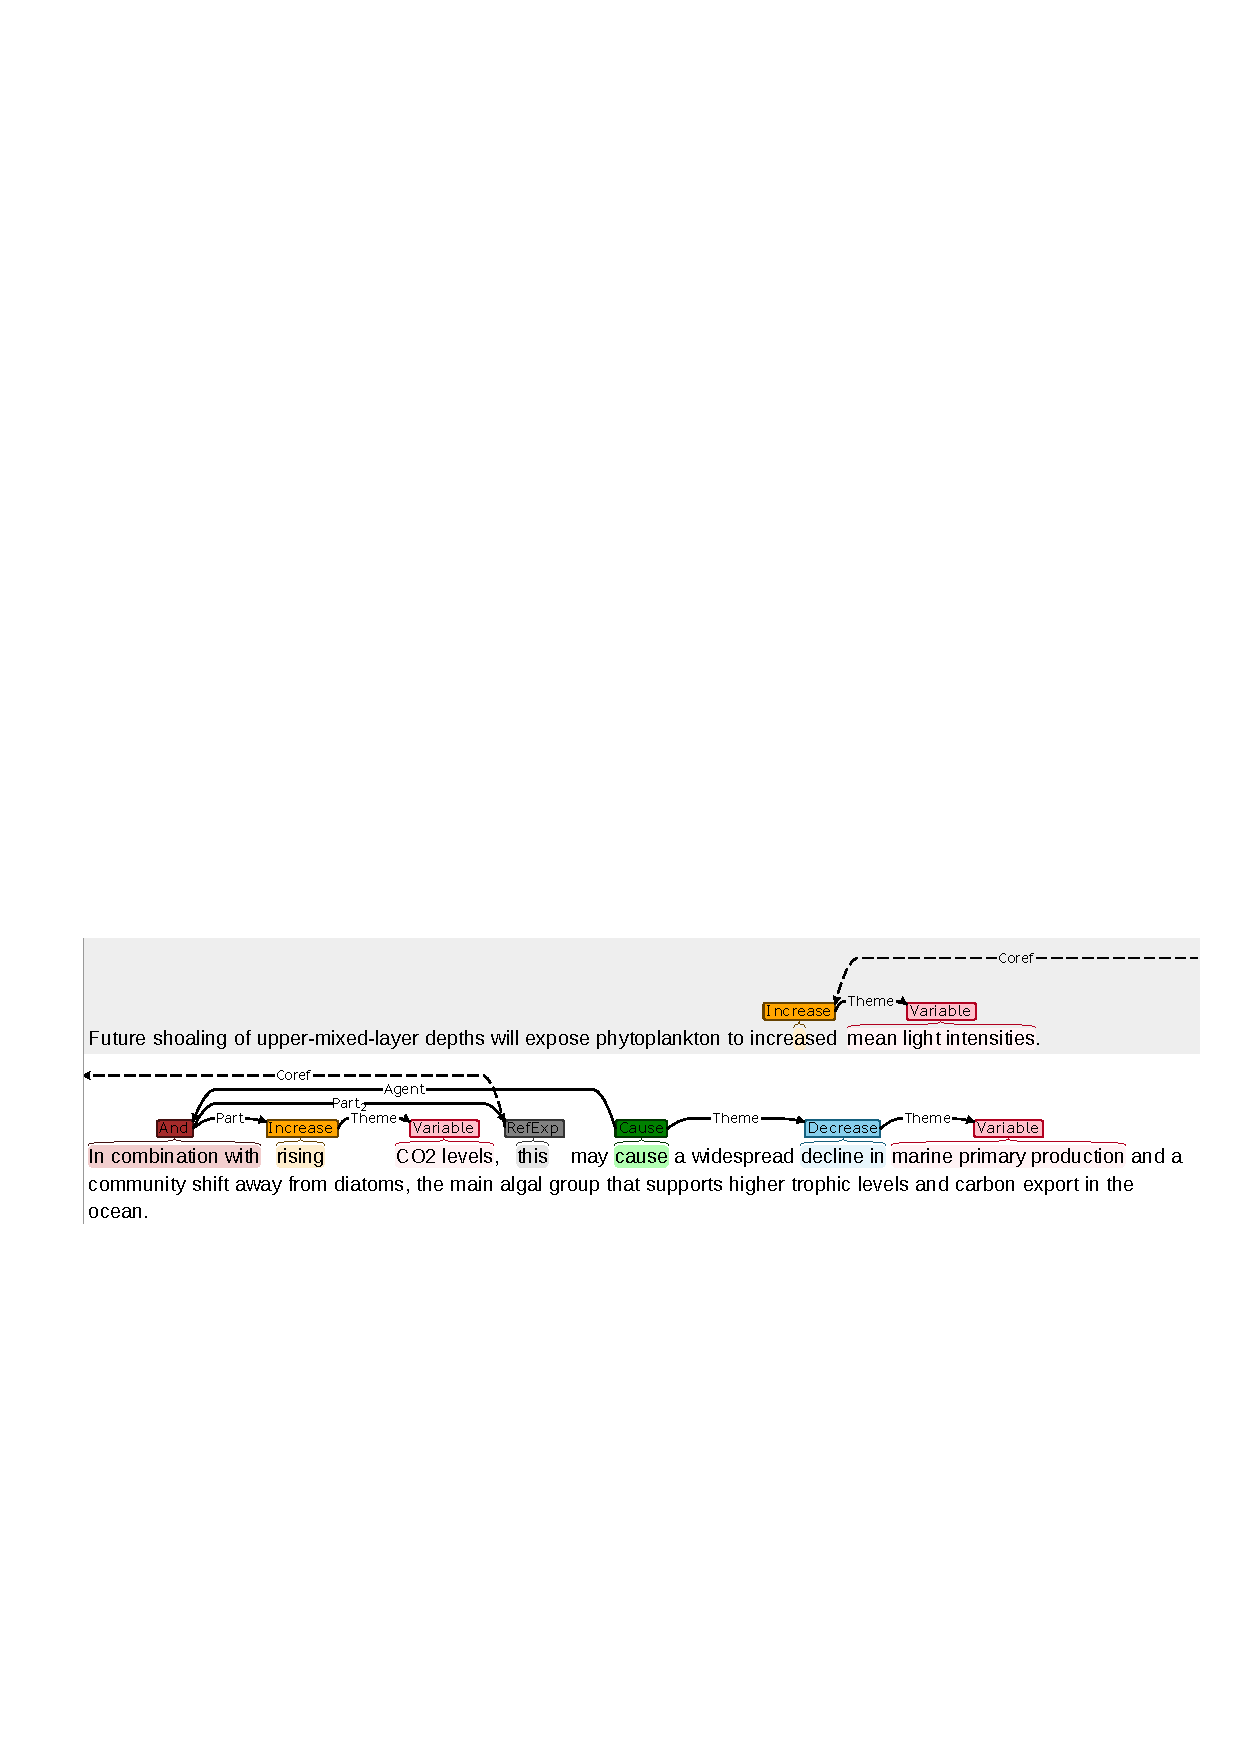
\includegraphics[scale=0.9]{ex1.pdf}}
\framebox[\textwidth]{[ $\uparrow$ mean light intensities $\wedge$ $\uparrow$ CO2 levels ]~~~ $\Longrightarrow$~~~$\downarrow$ marine primary production}
 \caption{Example of a causal rule extracted from a pair of annotated sentences}
\end{center}
\label{fig:ex1}
\end{figure*}


\begin{figure*}
\begin{center}
\framebox[\textwidth]{
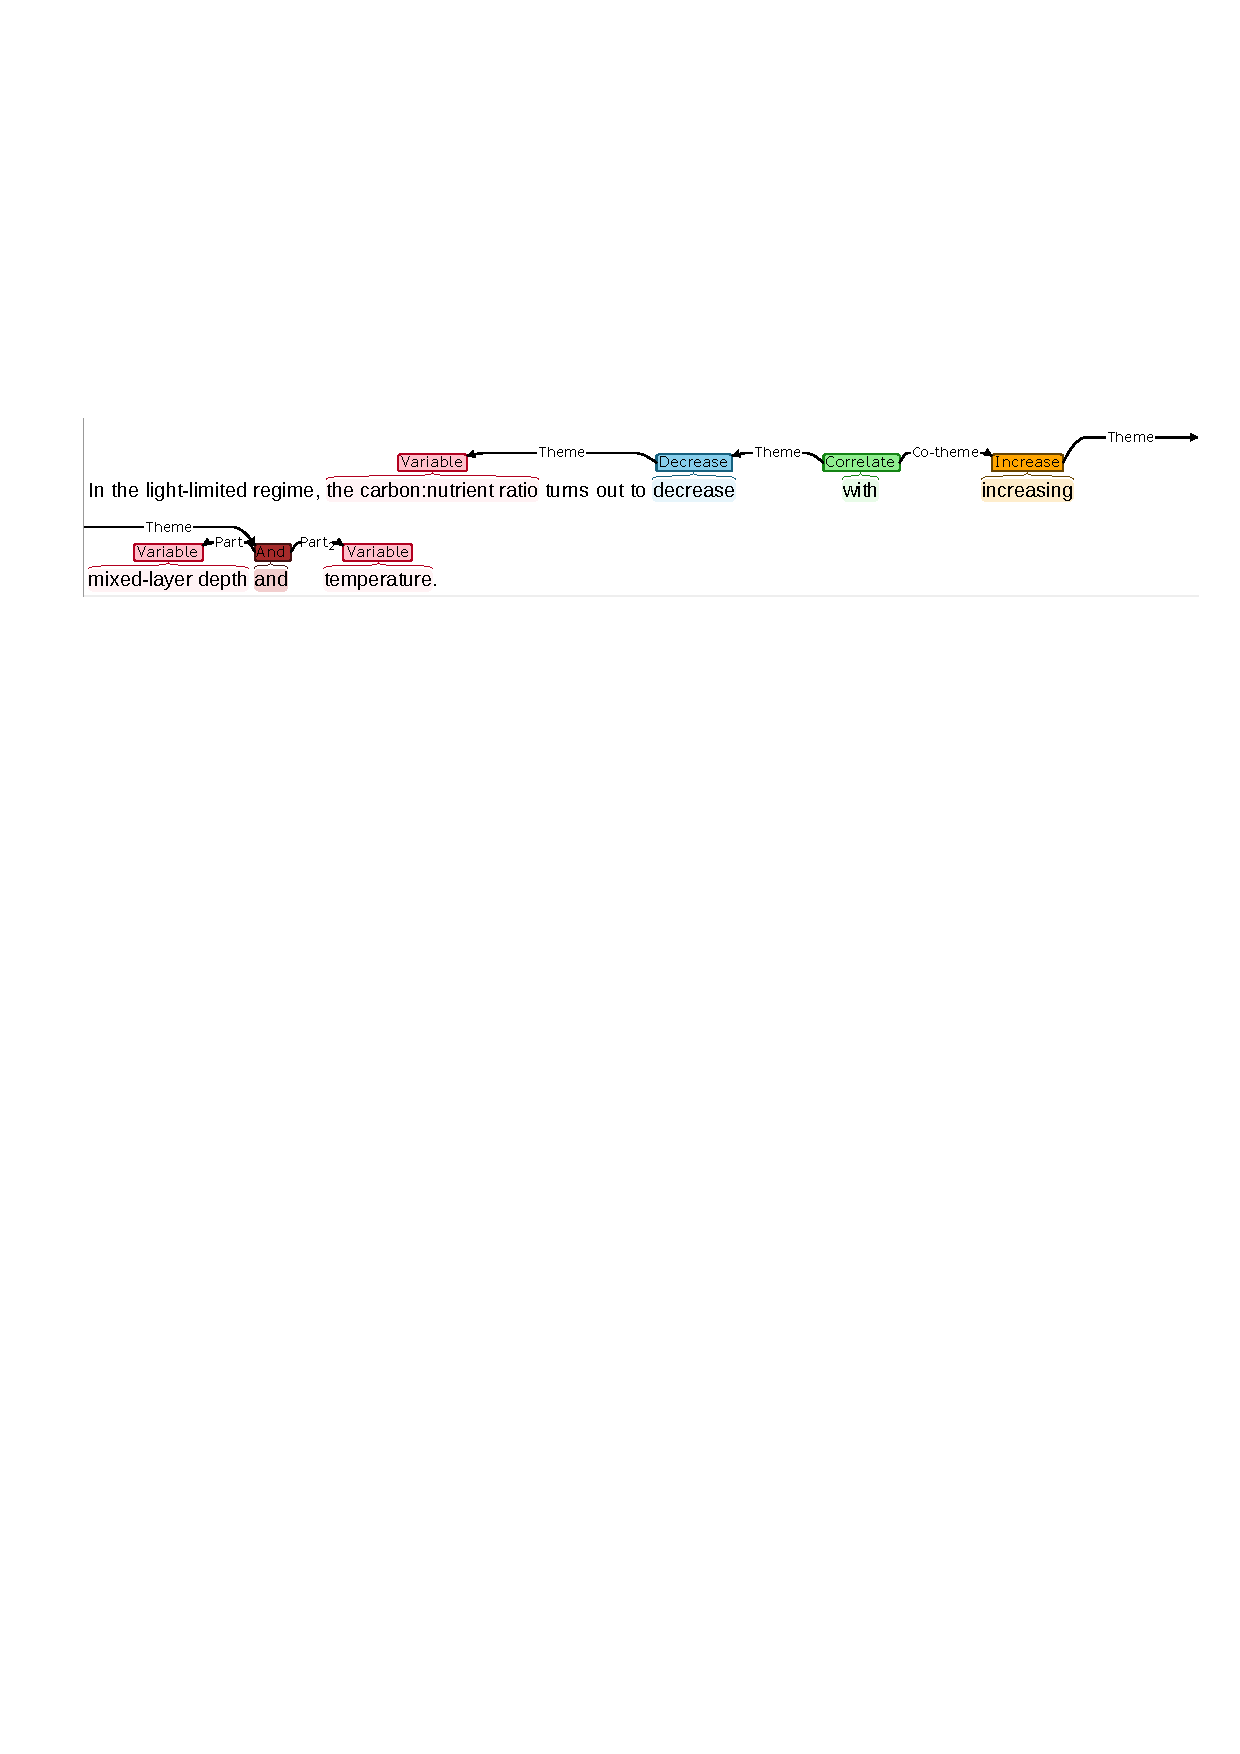
\includegraphics[scale=0.9]{ex2.pdf}}
\framebox[\textwidth]{[ $\uparrow$ mixed-layer depth $\wedge$ $\uparrow$ temperature ]~~~ $\leadsto$~~~$\downarrow$ the carbon:nutrient ratio}
 \caption{Example of a correlation rule extracted from an annotated sentence}
\end{center}
\label{fig:ex2}
\end{figure*}



\begin{figure*}
\begin{center}
\framebox[\textwidth]{
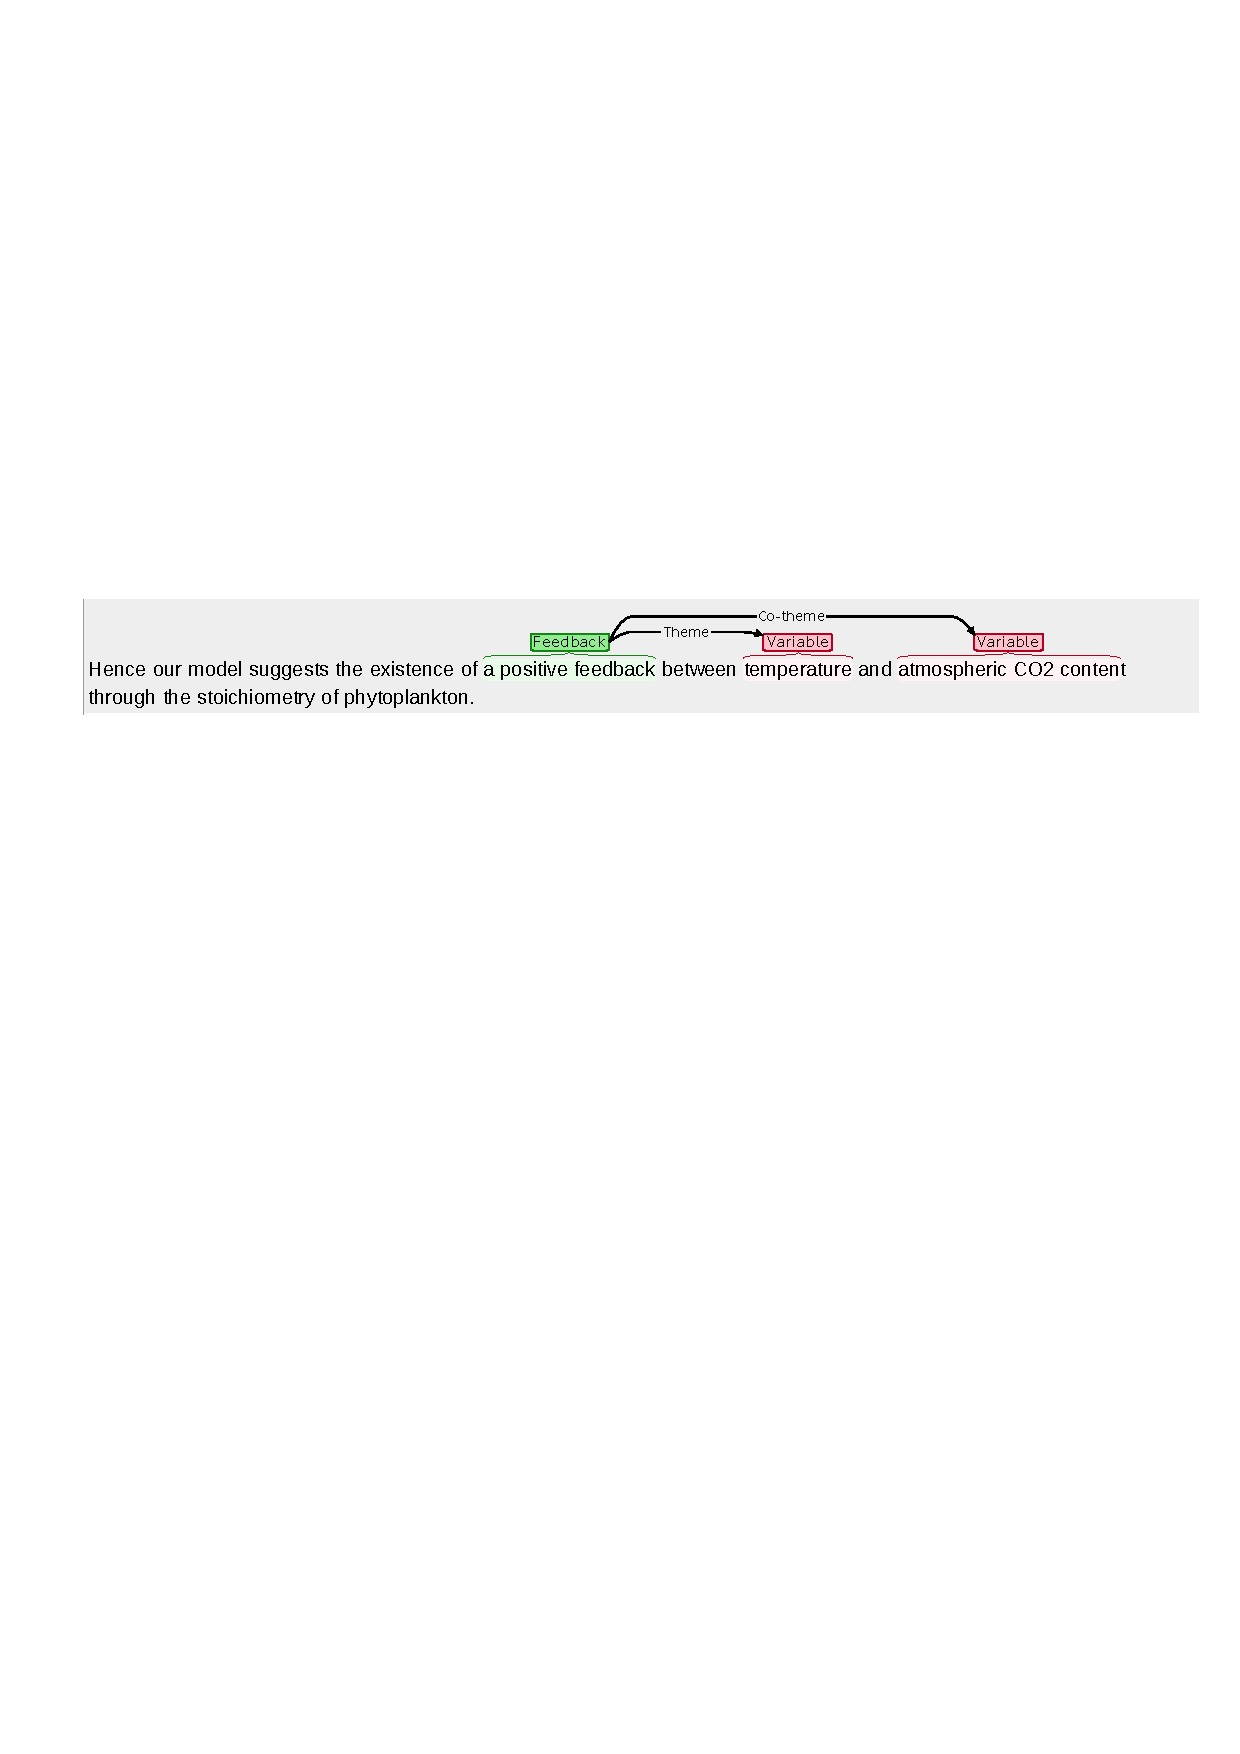
\includegraphics[scale=0.9]{ex3.pdf}}
\framebox[\textwidth]{$\updownarrow$ temperature~~~$\Longleftrightarrow^{+}$~~~$\updownarrow$ marine primary production}
 \caption{Example of a feedback rule extracted from an annotated sentence}
\end{center}
\label{fig:ex3}
\end{figure*}


%=============================================================================
\section{Discussion}
%=============================================================================
\label{sec:discussion}
 
The annotation scheme proposed below seems a good candidate for the pupose of rule extraction.
However, it has only been tried on a small set of abstracts and it remains to be seen how it holds up when applied to more text.
Inter-annotator agreement has not been measured so far.
In addition to this, we are also considering a type of evaluation in which extracted rules and their corresponding source texts are shown to domain experts, who are then asked to judge to what extent the rule is entailed by the text. 

\todo[inline]{Automatic annotation:
What aproach do we intend to use?
Generic, unsupervised open IE vs dedicated supervised system?
How well do we think this is going to work?
Bootstrapping and active learning to save annotation costs?
}

The extracted rules expressing relations of correlation, causality or feedback between quantitative variables are intended to be used in knowledge discovery support systems.
One use case is to search for other variables directly related to a certain variable of interest.
For example, find all processes that affect or are affected by a rise in atmospheric CO2 level.
The variable in question may be expressed in many different ways though, for example, as \emph{CO2}, \emph{atmospheric CO2}, \emph{CO2 concentrations} or \emph{CO2 partial pressures}, but not as \emph{ CO2 levels in oceanic surface waters} or \emph{the distribution of CO2 between the atmosphere and the ocean}.
Simple string matching between the variables in queries to those in rules will given limited recall and precison.
Related to this is the issue of differences in terminology across research fields.
For instance, \emph{export production} and \emph{biological pump} are different terms, used by chemists and biologists repspectively, for the same process of carbon cycling in the oceans. 
One possible strategy to cope with this issue is to normalize all relevant entities by linking them to a unique concept in an ontology \cite{Bada2012Concept}.
However, whereas the concepts of interest in biomedicine are relatively well understood -- including entities such cells, proteins and genes -- and covered by widely used ontologies, earth science currently seems to lack a similar common ground.

A different but related problem is exemplified in correlation rule \Next[b] extracted from the second part of sentence \Next[a].

\exi. 
  \a. Concentrations of DFe increased slightly with depth in the water column, while that of TaLFe did not show any consistent trend with depth.
  \b. $\neg$ [ $\updownarrow$ depth~~~$\leadsto$~~~$\updownarrow$ that of TaLFe ]

The problem is that \emph{depth} in \Last[b] is too general and should in fact be linked to \emph{depth in the water column} for proper interpretation. 
Likewise, \emph{that of TaLFe} should be interpreted as \emph{concentrations of TalFE}.
This illustrates the need for coreference resolution and more general, linking of subsequent mentions of the same entity in the text, a notoriously hard task in NLP. 

Another use case for extracted rules is to generate potential hypotheses about indirect relations between variables or feedback loops.
This can be accomplished by chaining together two or more rules, matching the change event on the right-hand-side of one rule to a similar change event on the left-hand-side of another rule.
Matching gives rise to the same problems discussed above, i.e., different ways of referring to the same entity.
In addition, there is the issue of context-dependency.
Most rules are not universally applicable, but only apply under certain conditions in a particular context.
For example, a rule may be limited in scope to certain biological species or organisms, a particular geographical region or historical time period, subject to a given assumption (\emph{only if \ldots}), etc.
This is related to initiatives for annotating meta-knowledge such as confidence level (fact vs. conjecture), source (observation vs. analysis) or origin (present or cited work) as in  \cite{Thompson2011Enriching}.  
Proper modelling of rule context would require a rather deep understanding of the whole text. 
For now, we plan to leave this to the user by offering facilities in the user interface to quickly inspect the source text for each rule.

Inference with rules may be further enhanced by exploiting domain knowledge.
For example, given an ontology which contains the fact that \emph{diatoms} are a kind of \emph{phytoplankton}, rules containing either of the terms may be generalized by substituting the hypernym or specialized by substituting the hyponym.
In a similar vein, rules can be generalized by removing specifiers, modifiers or parts of a conjunction.
Whether or not this constitutes valid inference seems connected to recent developments in textual entailment, in particular work on natural logic \cite{MacCartney2008Modeling}.
    

%=============================================================================
\section{Conclusion}
%=============================================================================
\label{sec:conclusion}

An annotion scheme was proposed to capture events of change, cause, correlation and feedback, as well as  the entities involved in them, in the cross-disciplinary domain of earth science, environmental science and climate science.
It was shown that rules about the relation between changing processes can be automatically extracted from annotated text.
Follow up work will involve annotating more text, measuring interannotator agreement and rule adequacy.
Next, tools for automatic annotation will be developed.
Future work will also address normalization of entities, tracking of entity mentions, modelling of rule context and combination with domain knowledge. 

 
%=============================================================================
\section{Acknowledgements}
%=============================================================================

\todo[inline]{
Financial aid from the European Commission (OCEAN-CERTAIN, FP7-ENV-2013-6.1-1; no: 603773) is gratefully acknowledged. 
}

\bibliographystyle{lrec2006}
\bibliography{biotxtm14}

\end{document}

